%
% einleitung.tex -- Beispiel-File für die Einleitung
%
% (c) 2020 Prof Dr Andreas Müller, Hochschule Rapperswil
%%
\section{Was ist ein Erdbeben? \label{erdbeben:section:teil0}}
\rhead{Erdbeben}
Für das Verständnis möchten wir zuerst erklären, was ein Erdbeben genau ist.
Das soll uns helfen, eine Verknüpfung zwischen dem Naturphänomen und der mathematischen Problemstellung herzustellen.

Unter einem Erdbeben verstehen wir eine Erschütterung des Erdkörpers.
Dabei reiben zwei tektonische Platten aneinander, welche sich durch die Gesteinsverzahnung gegenseitig blockieren.
Diese Haftreibung durch die Steine wird so lange aufgebaut, bis sie nicht mehr gehalten werden kann.
Wenn dies passiert, entlädt sich die aufgebaute Spannung und setzt enorme Energien frei, die wir als Erdbeben wahrnehmen.
Ein Erdbeben breitet sich vom Erdbebenherd in allen Richtungen gleich aus.
Vergleichbar ist, wenn man einen Stein in einen Teich wirft und die Wellen beobachten kann, die sich ausbreiten.

\subsection{Funktion eines Seismograph}
Um ein Erdbeben kenntlich zu machen, werden in der Regel Seismographen mit vielen Sensoren verwendet. 
Ein Seismograph besteht im Grunde aus einer federgelagerten Masse. Wirkt eine Bodenerregung auf das Gerät ein, schwing das Gehäuse und dadurch auch die gekoppelte Masse. 
Stoppt das Erdbeben, schwingt das Gehäuse nicht mehr. 
Die Masse schwing jedoch in seiner Eigendynamik weiter. 
Relativbewegung des Bodens kann damit als Auslenkung im Zeitverlauf gemessen werden.
In modernen Seismographen wird die Bodenbewegung in alle Richtungen gemessen, sowohl Horizontal als auch Vertikal. 
Wir konstruieren uns eine einfachere Version eines Seismographen mit eine Gehäuse, an dem zwei Federn und eine Masse befestigt sind. 
Der Seismograph ist in Abbildung ~\ref{erdbeben:Seismograph} ersichtlich.
Ein Sensor unter der Masse misst die Position, bzw. die Auslenkung der Feder und der Masse.
Dies bedeutet, unser Seismograph kann nur in eine Dimension Messwerte aufnehmen. 

\begin{figure}
 \begin{center}
 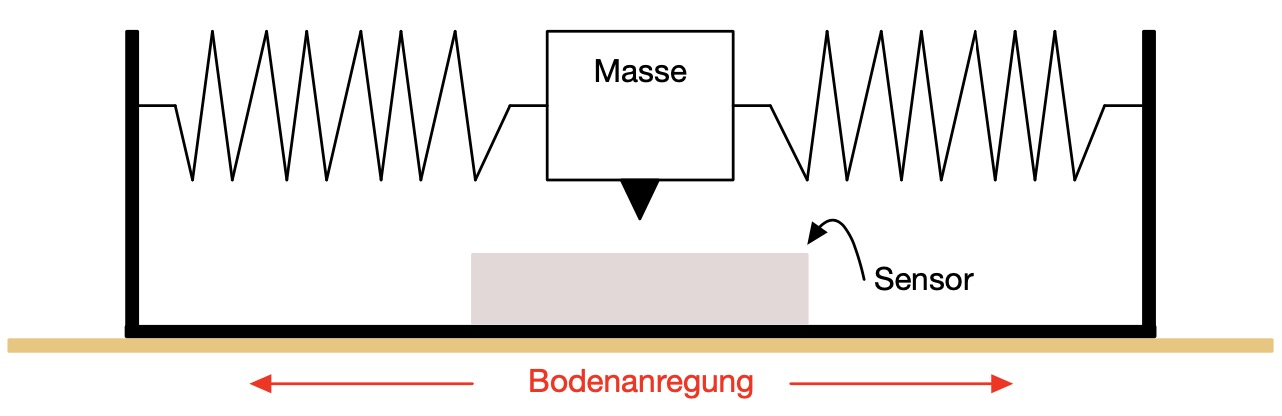
\includegraphics[width=5cm]{papers/erdbeben/Apperatur}
 \caption{Aufbau des Seismographen mit Gehäuse, Masse, Federn und Sensor}
 \label{erdbeben:Seismograph}
 \end{center}
\end{figure}

\subsection{Ziel}
Unser Seismograph misst nur die Position der Masse über die Zeit. 
Wir wollen jedoch die Beschleunigung $a(t)$ des Boden, bzw. die Kraft $f(t)$, welche auf das Gehäuse wirkt, bestimmten.  
Anhand dieser Beschleunigung, bzw. der Krafteinwirkung durch die Bodenbewegung, wird später das Bauwerk bemessen.
Dies bedeutet, die für uns interessante Grösse $f(t)$ wird nicht durch einen Sensor erfasst. 
Jedoch können wir durch zweifaches ableiten der Positionsmessung $s(t)$ die Beschleunigung der Masse berechnen. 
Das heisst: Die Messung ist zweifach Integriert die Kraft $f(t)$ inklusive der Eigendynamik der Masse.
Um die Krafteinwirkung der Masse zu berechnen, müssen wir Gleichungen für unser System finden.

\subsection{Systemgleichung}
Im Paper~\cite{erdbeben:mendezmueller} wurde das System gleich definiert und vorgegangen. 
Im Fall unseres Seismographen, handelt es sich um ein Feder-Masse-Pendel.
Dieser kann durch die Differentialgleichung zweiter Ordnung einer gedämpften Schwingung am harmonischen Oszillator beschrieben werden. 
Die Gleichung lautet:
\begin{equation}
m\ddot s + 2k \dot s + Ds = f.
\end{equation}
wobei $m$ die Masse, $k$ die Dämpfungskonstante und $D$ die Federkonstante bezeichnet.
Da die Differentialgleichung linear ist, kann sie in die kompaktere und einfachere Matrix-Form umgewandelt werden.
Dazu verwenden wir die Subsitution:
\[ 
s_1 = s 
\qquad \text{und} \qquad
s_2 = \dot s
.
\]
Somit entstehen die Gleichungen für die Position $ \dot s_1(t)$ der Masse :
\[ \dot {s_1} = {s_2}\] 
und
\[ \dot s_2 = -\frac{D}{m} {s_1} -\frac{2k}{m} {s_2} + \frac{f} {m} \] 
für die Beschleunigung $\dot s_2(t)$ der Masse.
Diese können wir nun in der Form
\[ f =-\frac{D}{m} {s_1} -\frac{2k}{m} {s_2} + \frac{f} {m} \]
auch als Matrix-Vektor-Gleichung darstellen.
Dafür wird die Gleichung in die Zustände aufgeteilt. 
Die für uns relevanten Zustände sind die Position der Masse, die Geschwindigkeit der Masse und die äussere Beschleunigung des ganzen Systems. 

Dabei muss unterschieden werden, um welche Beschleunigung es sich handelt.
Das System beinhaltet sowohl eine Beschleunigung der Masse (innere Beschleunigung) als auch eine Beschleunigung der ganzen Apparatur (äussere Beschleunigung). 
In unserem Fall wird die äusseren Beschleunigung gesucht, da diese der Erdbebenanregung gleich kommt.
Dazu wird ein Zustandsvektor definiert:
\[ 
 \left(\begin{array}{c} {s_1} \\ {s_2} \\ {f} \end{array}\right).
 \] 
Durch Rücksubstituion ergibt sich uns folgende Systemgleichung in Matrix schreibweise, , wobei $\dot {s_1}= v$ ist:
\begin{equation}
\frac{d}{dt} \left(\begin{array}{c} s(t) \\ v(t) \\ f(t) \end{array}\right) = \left(
 \begin{array}{ccc} 	
0 & 1& 0 \\ 
- \frac{D}{m} &-\frac{2k}{m} & \frac{1} {m}\\
0 & 0 & 0\\
\end{array}\right)  \left(\begin{array}{c} s(t)\\ v(t)\\ f(t) \end{array}\right).
\end{equation}
Wir wissen nicht wie sich die Kraft verhält. 
Deshalb treffen wir die Annahme, das sich die Kraft über die Beobachtungszeit nicht verändert.
Diese Annahme ist nicht zulässig, jedoch ist dies das beste, was wir Annehmen können. 
Diese unzutreffende Annahme wird späteren Berechnungen berücksichtigen werden
Da die Kraft unbekannt ist, wird die letzte Zeile mit Nullen gefüllt, denn genau diese Werte wollen wir. 











